% Schema del modello definito in 05_layernorm.py, nella configurazione 'big':
% il GPT completo, disegnato nello stile della Figura 1 di "Attention Is All
% You Need" (di cui questo e' la meta' destra, il decoder).
%
% Rispetto allo schema del file 04 le novita' sono i LayerNorm - in versione
% pre-norm, cioe' PRIMA di ogni sotto-livello e non dopo come nella figura
% originale - piu' quello finale prima di lm_head, e il dropout.
%
% I numeri sono quelli della configurazione 'big'. Con 'small' diventano
% n_embed=32, 4 teste da 8, 3 layer, contesto 8, dropout 0.
%
% Compilare con:
%     pdflatex 05_out_architecture.tex
%     tectonic 05_out_architecture.tex

\documentclass[tikz,border=8pt]{standalone}

\usepackage[T1]{fontenc}
\usepackage{lmodern}
\usetikzlibrary{positioning,fit,calc,arrows.meta,backgrounds}

% i colori pastello della figura originale
\definecolor{cEmb}{RGB}{248,214,216}
\definecolor{cAtt}{RGB}{252,224,187}
\definecolor{cFF}{RGB}{200,225,245}
\definecolor{cLin}{RGB}{216,214,238}
\definecolor{cSM}{RGB}{205,235,205}
\definecolor{cNorm}{RGB}{250,242,205}
\definecolor{cBlk}{RGB}{240,240,240}

\begin{document}
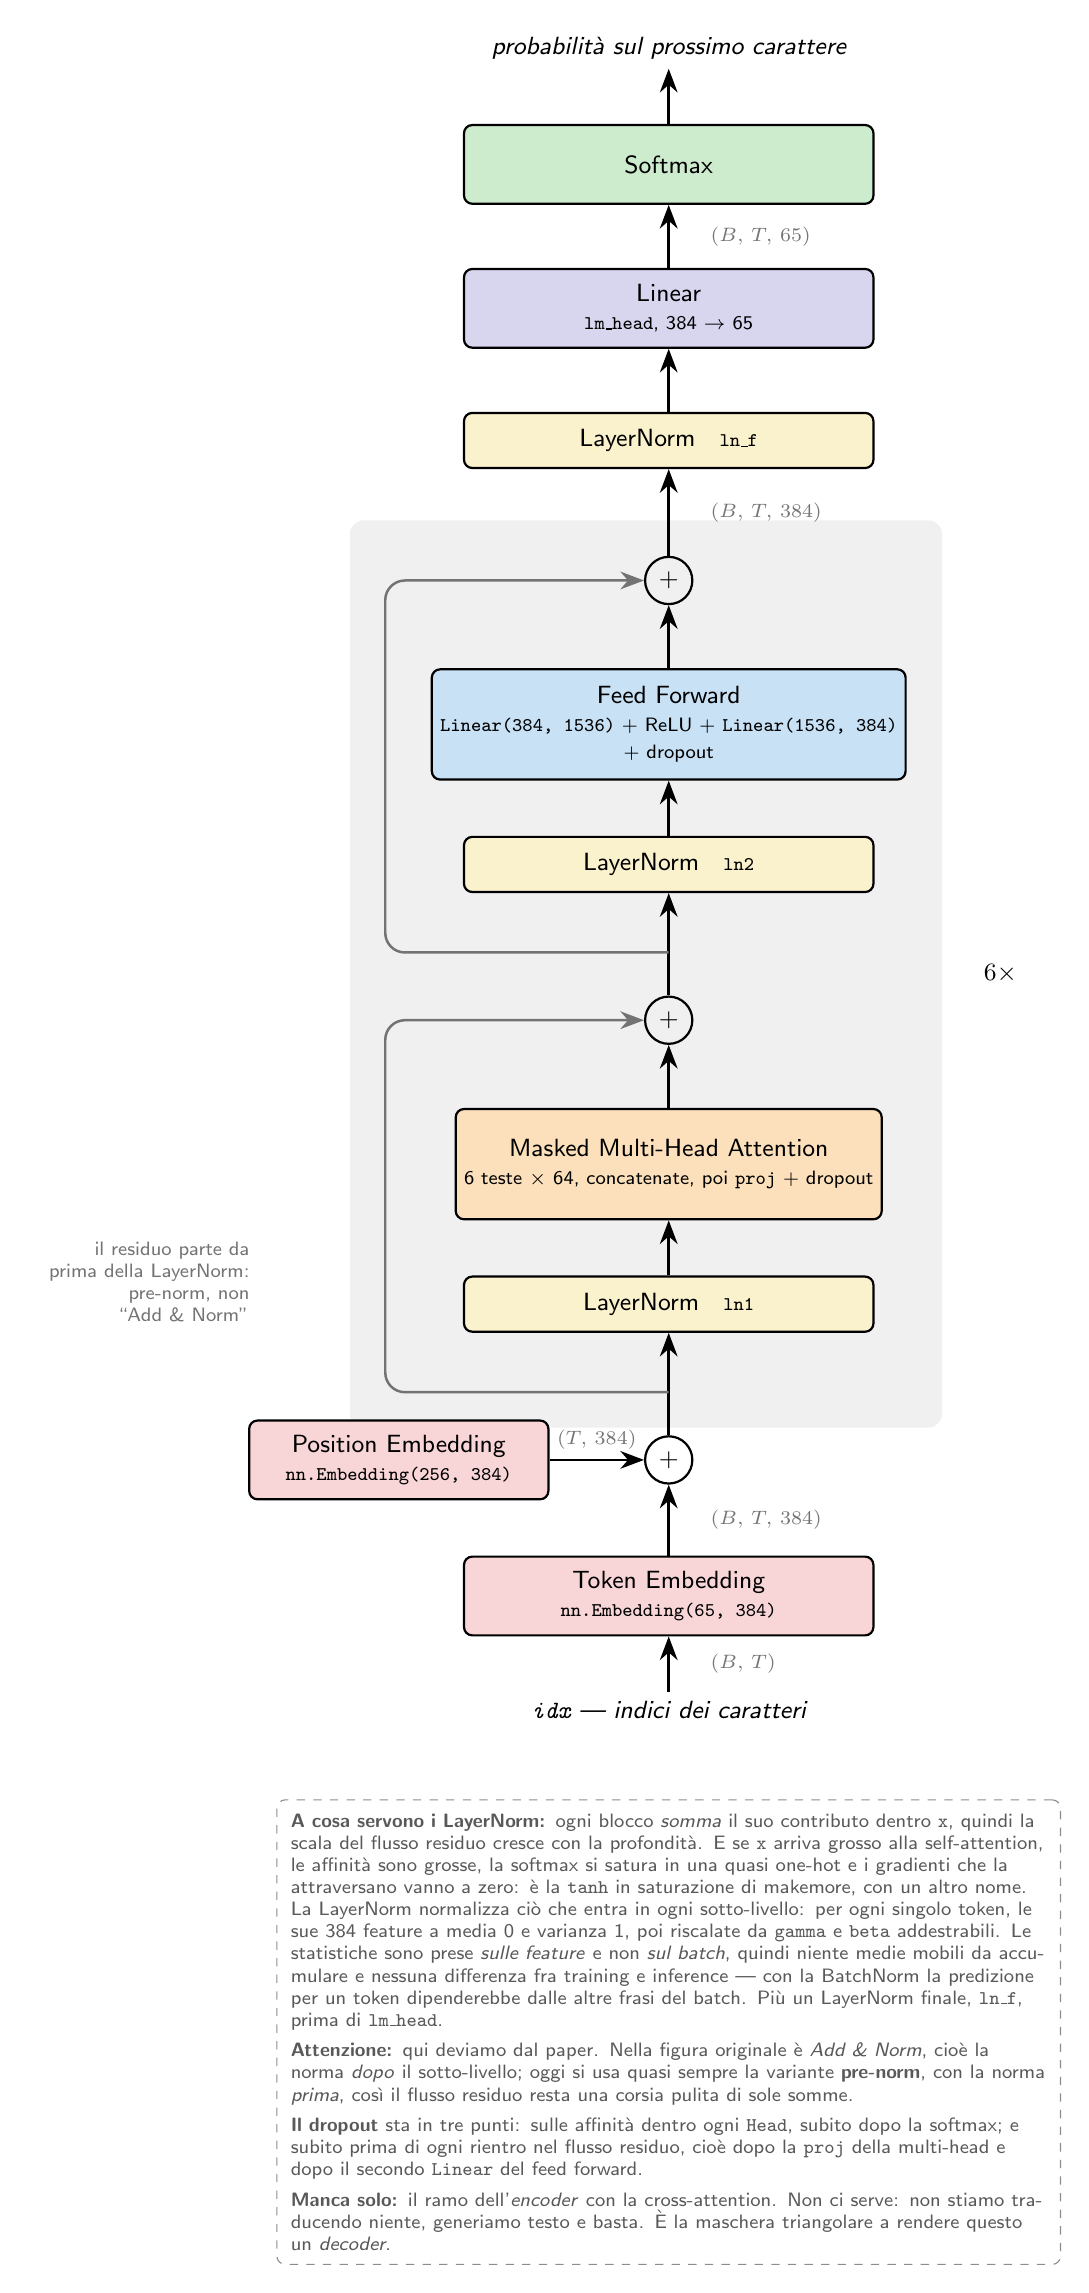
\begin{tikzpicture}[
  font=\sffamily\small,
  box/.style   = {draw, thick, rounded corners=3pt, align=center,
                  minimum width=52mm, minimum height=10mm, inner sep=3pt},
  norm/.style  = {box, fill=cNorm, minimum height=7mm},
  sum/.style   = {draw, thick, circle, minimum size=6mm, inner sep=0pt},
  io/.style    = {align=center, font=\sffamily\small\itshape},
  flow/.style  = {-{Stealth[length=3mm]}, line width=0.9pt},
  res/.style   = {-{Stealth[length=3mm]}, line width=0.9pt, black!55},
  shp/.style   = {font=\sffamily\scriptsize, text=black!55,
                  anchor=west, xshift=4mm},
  tag/.style   = {font=\sffamily\scriptsize, text=black!55},
  note/.style  = {draw=black!45, dashed, rounded corners=3pt, align=left,
                  font=\sffamily\scriptsize, text=black!65, inner sep=5pt}
]

% ---------------------------------------------------------------- il flusso --
\node[io]                                   (inp) {\texttt{idx} \textemdash{} indici dei caratteri};
\node[box, fill=cEmb, above=7mm of inp]     (tok) {Token Embedding\\[-1pt]{\scriptsize\texttt{nn.Embedding(65, 384)}}};
\node[sum, above=9mm of tok]                (add0) {$+$};
\node[box, fill=cEmb, left=12mm of add0,
      minimum width=38mm]                   (pos) {Position Embedding\\[-1pt]{\scriptsize\texttt{nn.Embedding(256, 384)}}};

% --- il Block, in versione pre-norm: la norma sta PRIMA del sotto-livello ---
\node[norm, above=13mm of add0]             (ln1) {LayerNorm \; {\scriptsize\texttt{ln1}}};
\node[box, fill=cAtt, above=7mm of ln1,
      minimum height=14mm]                  (mha) {Masked Multi-Head Attention\\[-1pt]{\scriptsize 6 teste $\times$ 64, concatenate, poi \texttt{proj} + dropout}};
\node[sum, above=8mm of mha]                (add1) {$+$};

\node[norm, above=13mm of add1]             (ln2) {LayerNorm \; {\scriptsize\texttt{ln2}}};
\node[box, fill=cFF, above=7mm of ln2,
      minimum height=14mm]                  (ff)  {Feed Forward\\[-1pt]{\scriptsize\texttt{Linear(384, 1536)} + ReLU + \texttt{Linear(1536, 384)}}\\[-1pt]{\scriptsize + dropout}};
\node[sum, above=8mm of ff]                 (add2) {$+$};

\node[norm, above=11mm of add2]             (lnf) {LayerNorm \; {\scriptsize\texttt{ln\_f}}};
\node[box, fill=cLin, above=8mm of lnf]     (lm)  {Linear\\[-1pt]{\scriptsize\texttt{lm\_head}, 384 $\rightarrow$ 65}};
\node[box, fill=cSM, above=8mm of lm]       (sm)  {Softmax};
\node[io, above=7mm of sm]                  (outp) {probabilit\`a sul prossimo carattere};

% ------------------------------------------------------------------- archi --
\draw[flow] (inp) -- (tok) node[shp, midway] {$(B,\,T)$};
\draw[flow] (tok) -- (add0) node[shp, midway] {$(B,\,T,\,384)$};
\draw[flow] (pos) -- (add0) node[tag, midway, above] {$(T,\,384)$};

% il residuo parte da PRIMA della LayerNorm: normalizziamo solo cio' che entra
% nel sotto-livello, il flusso residuo resta una corsia di sole somme
\coordinate (s1) at ($(add0.north)!0.42!(ln1.south)$);
\coordinate (s2) at ($(add1.north)!0.42!(ln2.south)$);
\coordinate (r1) at ([xshift=-36mm]s1);
\coordinate (r2) at ([xshift=-36mm]s2);

\draw[line width=0.9pt] (add0) -- (s1);
\draw[flow] (s1) -- (ln1);
\draw[res, rounded corners=2.5mm] (s1) -- (r1) |- (add1.west);

\draw[line width=0.9pt] (add1) -- (s2);
\draw[flow] (s2) -- (ln2);
\draw[res, rounded corners=2.5mm] (s2) -- (r2) |- (add2.west);

\draw[flow] (ln1) -- (mha);
\draw[flow] (mha) -- (add1);
\draw[flow] (ln2) -- (ff);
\draw[flow] (ff)  -- (add2);

\draw[flow] (add2) -- (lnf) node[shp, midway] {$(B,\,T,\,384)$};
\draw[flow] (lnf)  -- (lm);
\draw[flow] (lm)   -- (sm) node[shp, midway] {$(B,\,T,\,65)$};
\draw[flow] (sm)   -- (outp);

% ------------------------------------------------- il Block, ripetuto 6 volte --
\begin{scope}[on background layer]
  \node[fill=cBlk, rounded corners=5pt, fit=(ln1)(mha)(add1)(ln2)(ff)(add2)(r1)(r2),
        inner sep=4.5mm] (blk) {};
\end{scope}
\node[font=\sffamily\small, right=4mm of blk] {$6\times$};

% ------------------------------------------------------------- annotazioni --
\node[tag, anchor=east, text width=27mm, align=right]
  at ([xshift=-16mm, yshift=14mm]r1) {il residuo parte da\\prima della LayerNorm:\\pre-norm, non\\``Add \& Norm''};

% -------------------------------------------------------------- le note --
\node[note, below=9mm of inp, text width=96mm] (nota) {%
  \textbf{A cosa servono i LayerNorm:} ogni blocco \emph{somma} il suo
  contributo dentro \texttt{x}, quindi la scala del flusso residuo cresce con
  la profondit\`a. E se \texttt{x} arriva grosso alla self-attention, le
  affinit\`a sono grosse, la softmax si satura in una quasi one-hot e i
  gradienti che la attraversano vanno a zero: \`e la \texttt{tanh} in
  saturazione di makemore, con un altro nome. La LayerNorm normalizza ci\`o che
  entra in ogni sotto-livello: per ogni singolo token, le sue 384 feature a
  media 0 e varianza 1, poi riscalate da \texttt{gamma} e \texttt{beta}
  addestrabili. Le statistiche sono prese \emph{sulle feature} e non
  \emph{sul batch}, quindi niente medie mobili da accumulare e nessuna
  differenza fra training e inference --- con la BatchNorm la predizione per un
  token dipenderebbe dalle altre frasi del batch. Pi\`u un LayerNorm finale,
  \texttt{ln\_f}, prima di \texttt{lm\_head}.\\[3pt]
  \textbf{Attenzione:} qui deviamo dal paper. Nella figura originale \`e
  \emph{Add \& Norm}, cio\`e la norma \emph{dopo} il sotto-livello; oggi si usa
  quasi sempre la variante \textbf{pre-norm}, con la norma \emph{prima}, cos\`i
  il flusso residuo resta una corsia pulita di sole somme.\\[3pt]
  \textbf{Il dropout} sta in tre punti: sulle affinit\`a dentro ogni
  \texttt{Head}, subito dopo la softmax; e subito prima di ogni rientro nel
  flusso residuo, cio\`e dopo la \texttt{proj} della multi-head e dopo il
  secondo \texttt{Linear} del feed forward.\\[3pt]
  \textbf{Manca solo:} il ramo dell'\emph{encoder} con la cross-attention.
  Non ci serve: non stiamo traducendo niente, generiamo testo e basta. \`E la
  maschera triangolare a rendere questo un \emph{decoder}.};

\end{tikzpicture}
\end{document}
